\documentclass{book}
\usepackage{graphicx} % new way of doing eps files
%\graphicspath{../images}
\usepackage{rotating} % for sideways
\usepackage{multirow} % for \multirow
\usepackage{url}      % for \url
\usepackage{hyperref} % for \href
\usepackage{listings} % nice code layout
\usepackage[usenames]{color} % color
\definecolor{listinggray}{gray}{0.9}
\definecolor{graphgray}{gray}{0.7}
\definecolor{ans}{rgb}{1,0,0}
\definecolor{blue}{rgb}{0,0,1}
%\newcommand*\lstinputpath[1]{\lstset{inputpath=#1}}

% \Code{title}{label}{file}{language}
\newcommand{\Code}[4]{
%  \lstinputpath{../labs}
  \lstset{language={#4}}
  \lstset{backgroundcolor=\color{listinggray},rulecolor=\color{blue}}
  \lstset{linewidth=\textwidth}
  \lstset{commentstyle=\textit, stringstyle=\upshape,showspaces=false}
  \lstset{frame=tb}
  \lstinputlisting[caption={#1},label={#2}]{#3}
}
\newcommand{\CommandLine}[1]{
\vspace{.1in}\textbf{\texttt{{#1}}}\vspace{.1in}
}

\usepackage{floatflt}
%\usepackage{cscilabs}

\topmargin 0in
\textheight 8.5in
\textwidth 6.5in
\evensidemargin 0in
\oddsidemargin 0in

\renewcommand{\chaptername}{Lab}


\title{
{\Huge Baylor University} \\
\vspace{1in}
{\large Department of} \\
{\Large Electrical and Computer Engineering}\\
\vspace{1in}
{\Large BME/ELC 4372} \\
{\Huge Bioinstrumentation Laboratories} \\
}
\author{
Keith Schubert\\
Professor\\
Department of Electrical and Computer Engineering\\
Baylor University
}
\date{}

\makeindex

\begin{document}

\baselineskip=1.05\normalbaselineskip

\maketitle

\tableofcontents

%\listoffigures

%\listoftables

\pagenumbering{arabic}

\chapter{Raspberry Pi}

Over the course of this semester we will be building a variety of medical and biological sensors.  We will be using the Raspberry Pi as our microcomputer to control them, because of its ease of use, large number of IO pins, and tons of example code to build on.  In this lab we will be introducing the Raspberry Pi and how to use it.  I am going to try to do most things in Python, due to its simplicity and extensibility, but I can't guarantee we won't have to do a little programming in another language.

%All of our Raspberry Pi's have been set up for us by Ken Ulibari, so we all owe him a big thanks for the great job he did.  Should you ever need to install a Raspberry Pi of your own, or modify one of these, my short notes and commands examples are in Appendix~\ref{chapter:RPiRef}.
One thing I really want to bring to your attention is the use of \textbf{git}.  Git is a version control system (VCS), that was designed by Linus Torvalds to handle the development of Linux.  I will be maintaining a git repo at github, which means you will be able to clone it and do a pull any time you want to update it.  You do not have to use git, it just saves time and is a good skill to know for industry.

\section{GIT}

\CommandLine{mkdir code}

\CommandLine{cd  code}

\CommandLine{git clone \url{https://github.com/BaylorBMEELC4372BioInstrumentation/labs.git}}

\CommandLine{git clone \url{http://github.com/adafruit/Adafruit-Raspberry-Pi-Python-Code.git}}

\CommandLine{cd Adafruit-Raspberry-Pi-Python-Code}

\CommandLine{ls}

To update from the main repository, just do a pull

\CommandLine{git pull}


\section{Das Blinken LED}

\begin{itemize}
  \item Raspberry Pi (with keyboard, mouse, monitor, cobbler, and breadboard)
  \item 220$\Omega$ - 330$\Omega$ Resistor
  \item LED
\end{itemize}

First you need to assemble the circuit.  Hook up a wire from a gpio pin to the anode (long leg) of the diode, then connect the resistor to ground.  The resistor limits the current flow.  The Pi will output 3.3V and the diode will cause about a .7V drop resulting in a 2.6V drop left over.  The remaining 2.6V flowing through around 220$\Omega$ to 330$\Omega$ will result in around 10mV, which is enough to light the LED but not cause problems sinking or sourcing the current for the Pi.  Generally be careful with more than 20mV - 30mV for an IC.

Boot the Pi by plugging it in.  When the desktop appears, launch a terminal either from the menu or the terminal button.  Type the following line to edit the code to turn on and off with a timer.

\CommandLine{sudo nano \url{das_blinken_light.py}}

Note that nano is a small editor, hence the cute name.  You are welcome to use any editor you like.  You should see something that looks like Code~\ref{code:dbli}.  The only thing you have to edit is the gpio pin number to match the one you used, see Figure~\ref{fig:RPiGPIO}.

\begin{figure}\begin{center}
\caption{Raspberry Pi 2 General Purpose Input Output (GPIO) pinout.}\label{fig:RPiGPIO}
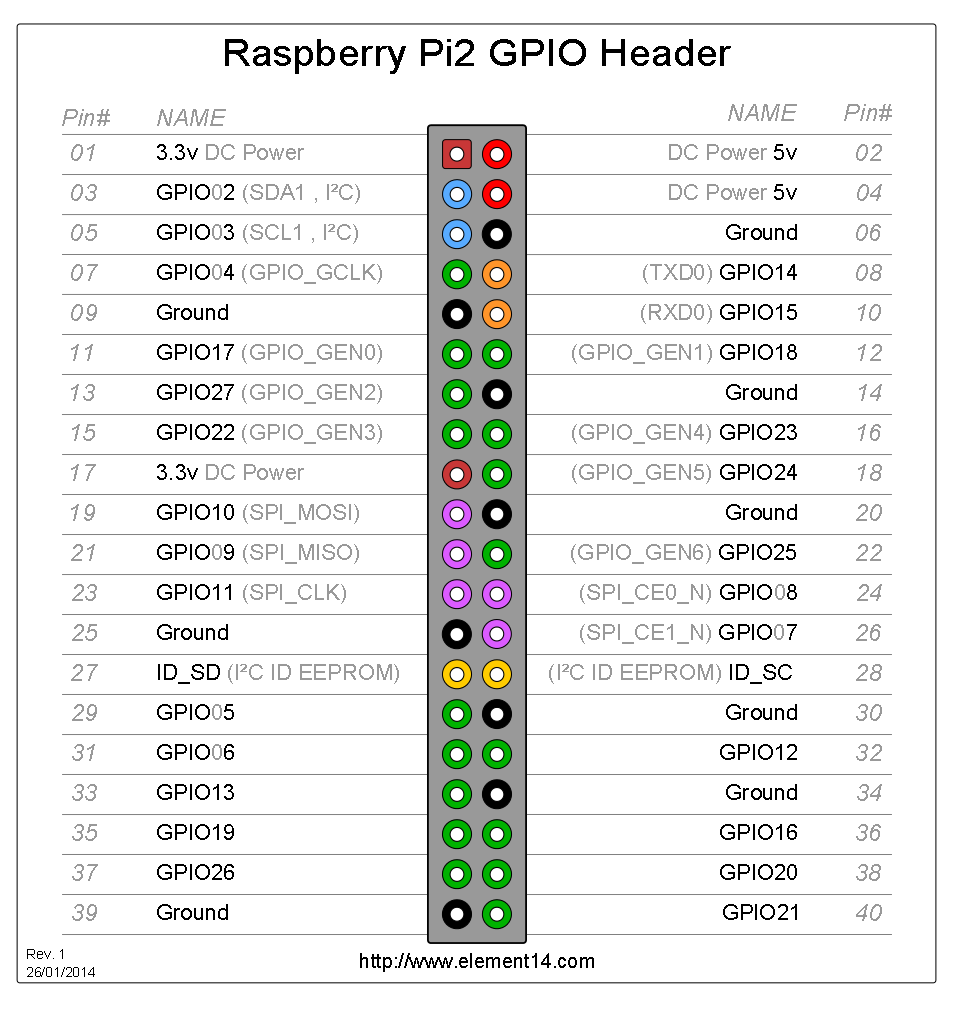
\includegraphics[width=.7\textwidth]{../images/GPIO_Pi2.png}
\end{center}\end{figure}

\Code{Blink the Light.}{code:dbli}{../labs/lab_01/das_blinken_light.py}{Python}

To run the code you need to type the following in the terminal window.

\CommandLine{sudo python \url{das_blinken_light.py}}

You need sudo to give enough permission to access the gpio pins.  The LED should blink on for a sec and off for a sec.

\section{Das Blinken LED II}

\begin{itemize}
  \item all the previous parts
  \item switch
\end{itemize}

Hook up with switch or button to ground.  The Broadcom chip that runs the gpio for the Pi has the ability to connect a pullup or pulldown resistor to an input.  We will thus use a pullup resistor, and the button will pull it down to ground when pressed.

We will now write code to read input and blink led if the button isn't pressed.  Type in:

\CommandLine{sudo nano \url{das_blinken_light_II.py}}

You can also refer to the GitHub repository, if need be.

\Code{Blink the Light while the button is not pressed.}{code:dblii}{../labs/lab_01/das_blinken_light_II.py}{Python}

\CommandLine{sudo python \url{das_blinken_light_II.py}}


\section{Das Blinken LED III}

One last thing for today is to dim the led.  The Raspberry Pi does not have an A/D converter, so we will just deal with two levels based on the button.  We also only have one pulse width modulated output on Broadcom (BCM) pin 18, which is Board pin 12.  Lack of A/D converters is one of several reasons it is not a replacement for a micro-controller, the main one being it doesn't have a real time operating system (RTOS) and lacks the necessary timers, like watchdog timers, to build one.  If you ever need a micro-controller then use an Ardino, MSP430, or similar.  The Pi has a bunch of advantages too in standard tools, quad core, and so on.  We care more about the later for labs and testing.  If you ever build patient used tools, get a micro-controller as you need the RTOS.

Getting back to the point, we want to have the LED on all the time now, and we will dim it when the button is pushed.  To handle the diming, we will use a pulse width modulator.  We will set the frequency to 50Hz, which is a reasonable refresh rate, and will use the duty cycle (percent of the wave that is high) to control the brightness.  This is a simple and standard way to handle this.  Type in:

\CommandLine{sudo nano \url{das_blinken_light_III.py}}

You can also refer to the GitHub repository, if need be.

\Code{Dim the Light while the button is pressed.}{code:dbliii}{../labs/lab_01/das_blinken_light_III.py}{Python}

\CommandLine{sudo python \url{das_blinken_light_III.py}}


\chapter{Electromyography (1A)}

\section{Biopotentials}

Biopotentials are formed by ion concentration differences inside and outside a cell.  Membranes and specialized pumps in the membrane regulate and adjust the concentrations in response to external and internal stimulation, permitting the generation and propagation of biosignals.  Measuring the electrical potential in muscles is called electromyography or EMG.


Generally, doctors use needle electrodes, so the skin only needs to be wiped with alcohol to prevent infection, but we will not be using needle electrodes for safety and legal reasons (Texas Court of Appeals, Third District, at Austin, Cause No. 03-10-673-CV. April 5, 2012)++.

\section{Setup}

First, we will get the Arduino IDE.  You  we need to make sure we have the latest version of our software.   Open a terminal window and enter the following commands:

\CommandLine{sudo apt-get update}

\CommandLine{sudo apt-get upgrade}

\CommandLine{sudo apt-get install arduino}

The ArduBerry is a shield that allows Raspbery Pi's to use Arduino shields.  Type the following commands:

\CommandLine{cd code}

\CommandLine{git clone https://github.com/DexterInd/ArduBerry.git}

Open a web browser and go to \url{http://www.dexterindustries.com/Ardubecrry/getting-started/} and follow the instructions.  You will download and install the drivers and run a simple test script that verifies everything is working.  The brief summary is below (the website has pretty pictures to accompany this):

\begin{enumerate}
\item Stack ArduBerry on Raspberry Pi.
\item Go to the scripts directory in the ArduBerry repo :\CommandLine{cd ArduBerry/script}
\item Make the install script executable:\CommandLine{sudo chmod +x install.sh} then run it as root: \CommandLine{sudo ./install.sh} and follow prompts, pressing \CommandLine{enter} and \CommandLine{y} as needed.
\item The system should automatically reboot.
\item Open the Arduino IDE from the system menu.
\item From the \textbf{Tools} menu, select the \textbf{Programmer} sub-menu, then select \textbf{RaspberryPi GPIO}.
\item Load \textbf{blink} or another sample sketch, and press \textbf{CTRL}$+$\textbf{Shift}$+$\textbf{U} to upload (or select \textbf{Upload using Programmer} from the File menu)
\item Verify that the LED blinks (if running blink)
\end{enumerate}

\subsection{Olimex EKG/EMG Shield}

You should not have to perform any installs for this.  The shield is static sensitive so be careful, and the pins are often bent so be more careful.  Disconnect power.  Insert onto the Arduberry. Connect power.  From Pi launch Ardino editor, and set the target device to an uno and the programmer to GPIO. \textbf{Load arduberry emg sketch}, then \textbf{program}.

Now open a command window and cd to your EMG directory.  Run EMG.py.  This is a simple test program, that should give you 8 numbers (1-4 interspersed with something around 300).  If you get this all is well.

Now connect a volunteer to the ekg leads.  L goes on the left arm, R goes on the right arm, and D goes on the right leg.  They need to be symmetrically placed, i.e. all at wrist/ankle or elbow/knee, etc.

Run either the fixed (takes 2k samples then plots and holds) or plot (for dynamic plots).

\section{General Advice}

Gel electrodes provide a good measure but a few basic precautions should be followed to get the best signals.

\begin{itemize}
  \item Remove oils from your skin with soap and water to improve the signal.
  \item Don't apply lotions or creams.
  \item Make sure you are hydrated (dry skin doesn't conduct as well).
  \item Try to use smooth skin with minimal hair (callouses and hair make it more difficult to get a good signal).
  \item Body fat reduces the signal, so try to find areas where the muscle is as close to the surface as possible.
\end{itemize}



\section{Test}

You will first need to setup the arduino on the shield to respond to our code.  From the application menu, pick the first menu group and the arduino ide should be the first pick.  In it, open the arduino sketch in our lab\_02 directory.  From the file menu select upload via programmer.  You are set.

Now open a terminal window and type

\CommandLine{cd c*/B*/l*/lab\_02}

\CommandLine{sudo python EMG\_plot.py}

After a second or two the plot window will open and start displaying the plot of the difference of R and L with D used as ground.  You can stop the plot with ctrl-c, though this will exit.  If you want to take a fixed data length and have the plot stay up then use

\CommandLine{sudo python EMG\_fixed.py}

I suggest using plot to try most of the experiments below.

Start with the metal plate electrodes.  Place ground on bicep.  Place the other two on the muscle the forearm that moves the wrist - one in the middle and one near the end.  What happens if you use the right leg?  Try metal plates and gel electrodes (just do arm)?

Place other two on the same forearm, one in the middle of a muscle and one near the end of the same muscle.  Locat muscles for two different fingers on the same hand by extending and contracting individually and noticing muscle flexure (i.e. I want you to do this twice).  What happens if you use the opposite arm  ?

Record signals for motion and identify finger flexed by chart only.  Explain.

How does the amount of exerted force relate to the signal? 
\chapter{Electro-Kardio-Gram}


\section{Setting up the Raspberry Pi}

\subsection{Adding the ArduBerry}

The ArduBerry is a shield that allows Raspbery Pi's to use Arduino shields.

Open a web browser and go to \url{http://www.dexterindustries.com/Ardubecrry/getting-started/} and follow the instructions.  You will download and install the drivers and run a simple test script that verifies everything is working.  The brief summary is below (the website has pretty pictures to accompany this):

\begin{enumerate}
\item Stack ArduBerry on Raspberry Pi.
\item Open terminal on the RPi, and cd to the code directory: \CommandLine{cd code}.
\item Clone the ArduBerry git repo: \CommandLine{git clone https://github.com/DexterInd/ArduBerry.git} and when it is finished go to the scripts directory in the ArduBerry repo :\CommandLine{cd ArduBerry/script}
\item Make the install script executable:\CommandLine{sudo chmod +x install.sh} then run it as root: \CommandLine{sudo ./install.sh} and follow prompts, pressing \CommandLine{enter} and \CommandLine{y} as needed.
\item The system should automatically reboot.
\item Open the Arduino IDE from the system menu.
\item From the \textbf{Tools} menu, select the \textbf{Programmer} sub-menu, then select \textbf{RaspberryPi GPIO}.
\item Load \textbf{blink} or another sample sketch, and press \textbf{CTRL}$+$\textbf{Shift}$+$\textbf{U} to upload (or select \textbf{Upload using Programmer} from the File menu)
\item Verify that the LED blinks (if running blink)
\end{enumerate}

\subsection{Olimex EKG/EMG Shield}

You should not have to perform any installs for this.  The shield is static sensitive so be careful, and the pins are often bent so be more careful.  Disconnect power.  Insert onto the Arduberry. Connect power.  From Pi launch Ardino editor, and set the target device to an uno and the programmer to GPIO. \textbf{Load arduberry emg sketch}, then \textbf{program}.

Now open a command window and cd to your EMG directory.  Run EMG.py.  This is a simple test program, that should give you 8 numbers (1-4 interspersed with something around 300).  If you get this all is well.

Now connect a volunteer to the ekg leads.  L goes on the left arm, R goes on the right arm, and D goes on the right leg.  They need to be symmetrically placed, i.e. all at wrist/ankle or elbow/knee, etc.

Run either the fixed (takes 2k samples then plots and holds) or plot (for dynamic plots).

\section{General Advice}

Gel electrodes provide a good measure but a few basic precautions should be followed to get the best signals.

\begin{itemize}
  \item Remove oils from your skin with soap and water to improve the signal.
  \item Don't apply lotions or creams.
  \item Make sure you are hydrated (dry skin doesn't conduct as well).
  \item Try to use smooth skin with minimal hair (callouses and hair make it more difficult to get a good signal).
  \item Body fat reduces the signal, so try to find areas where the muscle is as close to the surface as possible.
\end{itemize}
\chapter{Op Amps}

\section{MCP 3008}

The MCP 3008 is an 8 channel, 10 bit A/D converter that is bus addressable.  Communication is through a SPI bus.  Our Raspberry Pi has hardware support\footnote{If you had a controller that didn't have hardware support you would have to implement it in software, which is very slow and called bit banging.  I have included a bit banging code for your reference in the code part of lab 3.}.  There are four code sequences I have provided:
\begin{enumerate}
\item mcp3008bitbang.py - slow software SPI bus.  Don't use, this is only for reference if you don't have a system with hardware support.
\item mcp3008hw.py - fast hardware SPI bus.  outputs values on command line to 3 decimal places.  Good for getting precise values, but bad for lots of values.
\item mcp3008plot.py - hardware SPI bus that plots the results on a graph.  Tends to be slow because it has to sample and plot.
\item mcp3008plot-thread.py - multi-threaded hardware SPI bus that plots the result on a graph.  Yes I was having fun...  This has three threads, one that reads, one that outputs a square wave, and one that plots.  Syntax for the plot commands follows MatLab standards.  Fast and oh so much fun.
\end{enumerate}
These of course require library support so we have written an install shell script.  You will need to navigate to where it is located, change its permissions so it is executable, then run it.  From a terminal window type:

\CommandLine{cd ~/code/labs/labs}

\CommandLine{chmod 755 \url{install_python_libs.sh}}

\CommandLine{\url{./install_python_libs.sh}}

The mcp3008 has an analog power reference(Vref) and ground and a digital power (Vdd) and ground.  Vdd must always be connected to 3v3 (3.3V) and its ground (pin 9) to ground.  Vref and analog ground define the voltage range to compare.  Often this is the same, but it doesn't have to be.  For instance connecting to 5v gives a bigger swing.  Remember that the chip only has 10 bits of precistion (just over 1000 divisions) and thus the precision is:
$$
\frac{Vref-Agnd}{2^{10}}
$$
Thus the larger the reference swing, the less precise the measurement.  If you want to measure something small, you should have a small reference!  The basic hookup is thus

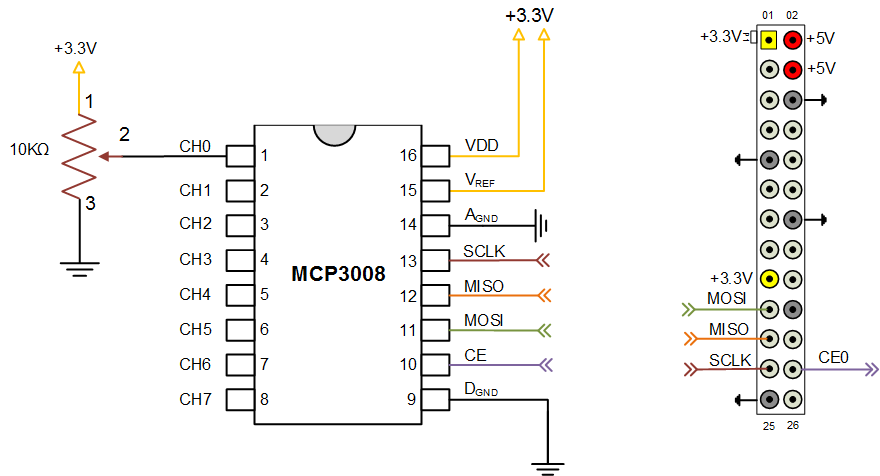
\includegraphics[width=0.8\textwidth]{../images/mcp3008_circuit.png} 

Note the voltage divider on the left is only for testing and does not need to be done each time.  You will build the divider the first time to test your code and setup.  The 8 pins on the left are now available for measuring your circuit.

\section{Follower}

We will be using a general purpose 741 Op Amp.  We will connect the positive rail to 3v3 and the negative rail to ground.  Hook the output to the negative input and the signal to follow goes on the positive input.  The pinout of the 741 is:

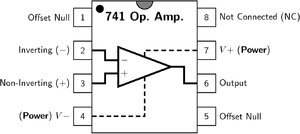
\includegraphics[width=0.4\textwidth]{../images/300px-Generic_741_pinout_top.png} 


\section{Inverting Amplifier}

Note we thus can't get negative voltages, but we have no choice since we don't have a negative voltage.  We can make a new reference ground by a voltage divider between 5v and ground with identical resistors (say around 1k each) or a potentiometer around a few k\footnote{hook 5v to one outer pin and ground to the other, the center tap is the reference}, so the center will be 2v5.  Hook this to the positive input, and the rails should be connected to 5v and ground.  Hook the Vref on the MCP3008 to 5v.  Now make another potentiometer voltage divider, this time running from the op amp's output to gpio 4, with the central tap going to the op amp's negative (inverting) input.




\chapter{One Wire Thermometer}

\section{Assemble Circuit}

The basic one wire temperature sensor from Dallas Semiconductor, uses a TO-92 package, just like a transistor.  Originally they only operated in parasitic mode, but the latest versions have had a powered version that can be run in parasitic mode. The pinout is as follows:

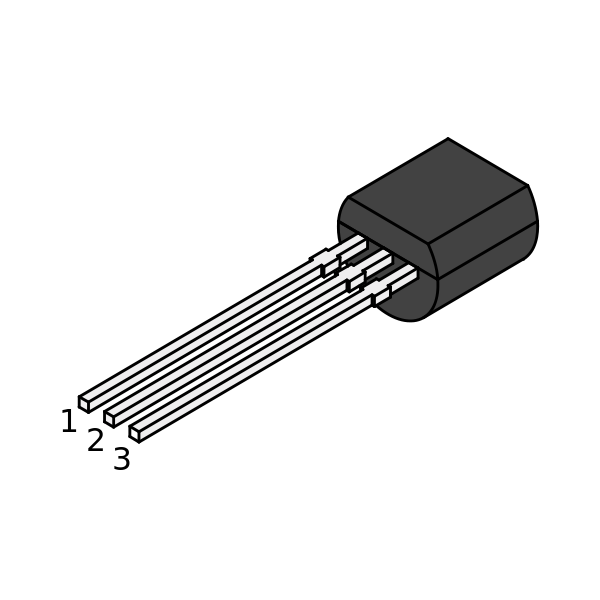
\includegraphics[width=0.4\textwidth]{../images/TO-92-Package.png}

where pin 1 is GND, pin 2 is the data line, and pin 3 is NC on old systems and 3.3v or GND on new ones (Ground for parasitic).  The data line needs a pull-up resistor\footnote{A resistor that supplies power to a bus, connected between the data and 3.3v in our case.} of around 3k$\Omega$ to 6k$\Omega$, with the sugested value at 4.7k$\Omega$. The one wire thermometer is very easy to connect to a Raspberry pi.  Connect pin 1 to ground, pin 2 to GPIO 4 (4th pin on the left of the Raspberry Pi's GPIO), and pin 3 to 3.3 volts.  Now connect a resistor around 4.7k$\Omega$ between pins 2 and 3 of the one wire.  You are ready to set up your Pi!

\section{Add One Wire Support}

First you need to edit the boot configuration file to add one wire support.

\CommandLine{sudo nano /boot/config.txt}

Scroll to the bottom (use the down arrow), then type \textbf{dtoverlay=w1-gpio}.
Save by typing \textbf{ctrl-o} then exit with \textbf{ctrl-x}.

Now reboot to make your changes active.


\CommandLine{sudo reboot}

\section{Test It}


\CommandLine{sudo modprobe w1-gpio}

\CommandLine{sudo modprobe w1-therm}



\CommandLine{cd /sys/bus/w1/devices}

\CommandLine{ls}

Note that the next directory has a really long name, and incorporates the device number so it is not constant on all systems.  This allows multiple to be connected.


\CommandLine{cd 28*}


\CommandLine{cat \url{w1_slave}}

\section{Code It}

\Code{Read from a One Wire Thermometer.}{code:w1}{../labs/lab_04/w1temp.py}{Python} 
\chapter{Pulse Oximeter (2B)}

\section{Background}
Hemoglobin is a protein in red blood cells that reacts to oxygen forming oxyhemoglobin (HbO$_2$).  When not oxygenated hemoglobin is referred to as deoxyhemoglobin (Hb).  Pulse oximetry is a non-invasive way to measure the amount of oxygen dissolved in the blood, which is called the oxygen saturation (SpO$_2$). Oxygen saturation is measured by detecting Hb and HbO$_2$, using their absorption sectra at two different frequencies (typically red around 660nm and infrared around 840nm to 940nm).  These values were selected because Hb has higher absorption of red light and HbO$_2$ has higher absorption of infrared, see figure~\ref{fig-spectrum}.

 \begin{figure}
 \caption{Absorption spectra of oxyhemoglobin and deoxyhemoglobin. \emph{Image by Adrian Curtin used under  Creative Commons Attribution-Share Alike 3.0 Unported License.}}
 \label{fig-spectrum}
 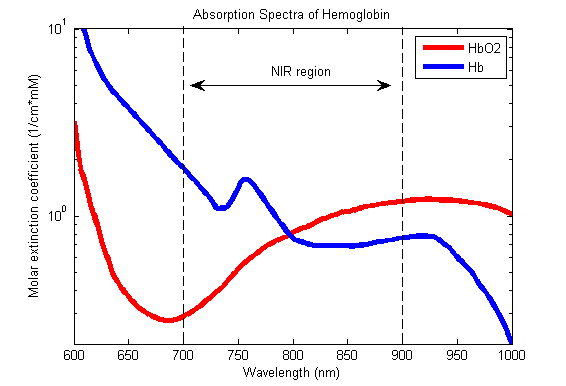
\includegraphics{../images/Oxy_and_Deoxy_Hemoglobin_Near-Infrared_absorption_spectra.png}
 \end{figure}

We are going to use two LEDs, one red one infrared, a photodiode, and a simple filter/amplifier to measure the absorbed light at two frequencies.  The data that produced the graph came from the tabulated molar extinction coefficient, e, for hemoglobin in water compiled by Scott Prahl using data from
\begin{itemize}
\item W. B. Gratzer, Med. Res. Council Labs, Holly Hill, London
\item N. Kollias, Wellman Laboratories, Harvard Medical School, Boston
\end{itemize}

\begin{tabular}{lrr}
$\lambda[ nm]$  & $HbO_2[ cm^{-1}/M]$ & $Hb[ cm^{-1}/M]$ \\
660              & 319.6                  & 3226.56 \\
830              & 974                    & 693.04 \\
840              & 1022                   & 692.36 \\
930              & 1222                   & 763.84 \\
940              & 1214                   & 693.44 \\
\end{tabular}

To get absorption, you multiply the molar extinction coefficient times the molar concentration times the pathlength and divided by the molecular weight of hemoglobin.  Since we are comparing two absorption measurements at different frequencies, the molecular weight of hemoglobin cancels and can be ignored.  Similarly, if we put both light sources (red and infrared) equally distant through your body to the photodiode, then the pathlength will also cancel and can be ignored.  %Let $x_{Hb}$ and $x_{HbO_2}$ be the concentration of deoxyhemoglobin and the concentration of oxyhemoglobin respectively, then the absorption is

Light is absorbed by tissue, venous blood, non-pulsatile arterial blood, and pulsatile arterial blood.  The first three are constant and will be measured as the DC component of the measurements.  The final one, pulsatile arterial blood, will be the AC component, and will also allow us to get heart rate.

\section{First Method}

By taking the ratio of oxygenated arterial blood in the pulsatile (AC) over the other (DC) portion of the signal at two frequencies we can calculate the absorption ratio (AR)\footnote{$SpO_2$ can also be calculated by ratio of the logarithms of the AC components at the two frequencies.  Multiply by 100 to get percent.}
\begin{equation}
AR = \frac{\frac{AC_{red}}{DC_{red}}}{\frac{AC_{infrared}}{DC_{infrared}}}
\end{equation}
We can then compare this number to previously measured values that were tested in a different manner.  This is only approximate because of differences in blood volume, perfusion, etc. as well as movement and misplacement effect measurements.  Even so we can make a simple table of values and interpolate to get other values:

\begin{tabular}{lr}
$AR$ & $SpO_2$ \\\hline
0.4  & 100\% \\
1.0  & 85\% \\
3.4  & 0\% \\
\end{tabular}


\chapter{Electro-Encephlogram}

%\chapter{Resistive Sensors}


\section{Fast and Cheap}




\Code{Measure resistive sensor by its time constant with 1uf capacitor.}{code:resistmtc}{resistive_measure_time.py}{Python}




\section{Analog to Digital Conversion}



%\appendix

%\chapter{Raspberry Pi Ref}\label{chapter:RPiRef}

\section{Preparing Your Pi}

The Raspberry Pi can use a variety of OS's, but its basic one is a Linux distro.

\begin{description}
  \item[sudo] runs the command after it as another user, who is by default the super user, hence the name Super User DO.
  \item[apt-get] patches and upgrades the system and applications.
\end{description}

sudo apt-get update %get the latest version

sudo apt-get upgrade %upgrade what you have to what you updated

sudo apt-get install git %install git, great way to get lots of code

sudo apt-get install python-dev %install python development

sudo apt-get install python-rpi.gpi %install python raspberry pi gpio tools

\section{getting code}

git clone http://github.com/adafruit/Adafruit-Raspberry-Pi-Python-Code.git

cd Adafruit-Raspberry-Pi-Python-Code

ls

\section{coding}

For Raspberry Pi

The simplest way to ensure some cleanup code gets run is to wrap your while loop in a try/finally block.

If you specifically want to catch Ctrl+C but nothing else, you can use try/except to catch KeyboardInterrupt.

Finally, if you want a more robust way to ensure some cleanup gets done, take a look at lines 312 through 322 in this revision of my Procrastinator's Timeclock utility.

https://github.com/ssokolow/timeclock/blob/3bb9889...

First, it assigns the cleanup function to sys.exitfunc so it'll get called on clean exit, then it hooks all the common POSIX signals the kernel might send s ensure that they trigger a clean exit.

* SIGINT is sent by Ctrl+C, which INTerrupts the program.
* SIGTERM is sent by things like task managers politely asking your program to TERMinate itself.
* SIGHUP is sent by the kernel when your program loses the terminal it's attached to.
* SIGQUIT is sent by Ctrl+\, which asks the program to quit and dump core if core dumping is enabled.

(My code technically doesn't handle SIGQUIT properly, since it doesn't dump core, but I've never seen people using it properly.)

Finally, it also uses try/except to catch Ctrl+C, just to play it safe. (And it's still not perfect because PyGTK doesn't let the program attach a handler for "lost connection to X server")

If you want a version that's a bit more complicated, but also works on Windows, look at this revision:

https://github.com/ssokolow/timeclock/blob/7a50500...

(It checks that each signal exists before hooking it)


\end{document}

